\chapter{Prototype and example usage}

\begin{chapterintro}
In this chapter we are going to describe a selected use case. It is going to be explained the running of all the tools involved and its purpose.
It is based on how to crawl the web to find new mashups, then feed the repository, do the validation and rejections of the mashups, and finally the developer will be able to use the discovered services.
\end{chapterintro}

\cleardoublepage

\section{Introduction}

In this use case 2 actors are involved, the administrator and the developer user.

\begin{table}[!htpb]
\centering
\begin{tabular}{|c|c|x{6cm}|}
\noalign{\hrule height 2pt}
\textbf{Actor identifier} & \textbf{Role} & \textbf{Description}\tn
\hline
ACT-1 & Admin & Administrator of the OMR, in charge of tasks such as inserting, deleting mashups, as well as including new available mashup repositories..\tn
\hline
ACT-2 & Developer & Technical developer which uses the OMR.\tn
\noalign{\hrule height 2pt}
\end{tabular}
\caption{Actors list}
\label{tab:actoresusecase}
\end{table}

The goal of the administrator is to provide the user the content that he needs. 

In this context, the developer is building a web application that consists of a social network in which users need to take photos and share them with other users. After sharing them, the photos need to be represented in a map. The developer wants to find an on-line service that already provides this functionality.

The developer user will query the repository using the OMR Web developer interface. The repository must have been fed up previously by an administrator, who doesn't know exactly the services that developers will need but he can think of which might be suitable for them.

To achieve the goals defined before we are going to follow the following steps. First of all launch scrappy to obtain all the web resources we need to feed the repository, once this has been done, the administrator user has to use de OMR admin interface in order to select the mash-ups that the developer user could possibly need for his application. The developer user will be able to find the mash-ups needed using the OMR Web developer interface.

In this scenario each module will run separately to demonstrate that they all can be standalone applications.

There is going to be a remote repository (OMR) located in Chemnitz University of Technology (Germany). The automated discovery process is done using one of the computers in the laboratory of Grupo de Sistemas Inteligentes. Both Administrative interface and developer interface will run in a web server located also in Grupo de Sistemas Inteligentes. The LMF will run in a separated server in the laboratory. This is resumed in table \ref{tab:executionenviroment}.


\begin {table}[h]
\caption {Execution enviroment} \label{tab:executionenviroment} 
\begin{center}
	\begin{tabular}{|c|r|}
		\hline \textbf{Component}                  	   & \textbf{where it runs}          \\ 
		\hline Omelette Mashup Registry (OMR)                  	   &   Chemnitz University of Technology, (Germany)       \\ 
		\hline Automated discovery service                 	   &   Laboratory, GSI (shannon.gsi.dit.upm.es)        \\
		\hline Ranking module 									&   Laboratory, GSI, (shannon.gsi.dit.upm.es)        \\ 
		\hline OMR Administrative interface                 	   &   Laboratory, GSI, (minsky.gsi.dit.upm.es)        \\ 
		\hline OMR Web developer interface                  	   &   Laboratory, GSI, (minsky.gsi.dit.upm.es)        \\
		\hline Linked Media Framework (LMF)                  	   &   Laboratory, GSI, (krusti.gsi.dit.upm.es)        \\ 
		\hline 
	\end{tabular} 
\end{center}
\end{table}

\newpage
\section{Automatic service discovery}
\label{sec:autodiscovery}

As explained in section \ref{sec:scrappy}, the discovery of new services and mashups is done using Scrappy.
Installation and configuration of Scrappy can be found in appendix \ref{apdx:installscrappy}.

The administrator user has to run Scrappy and insert the results into the OMR.
It is important to have configured the OMR endpoint in the config file as explained in appendix \ref{apdx:installscrappy}.

For this example we are going to scrap the sites of \textit{Programable Web}, \textit{Opera Widgets} and \textit{Yahoo Pipes}.

\begin{lstlisting}[style=consola, caption={Scrappy launching}]
scrappy -g programmableweb.com
scrappy -g pipes.yahoo.com
scrappy -g widgets.opera.com
\end{lstlisting}


By executing Scrappy it will directly feed the repository with services in RDF format like listing \ref{lst:fullexamplerdf}.

\begin {table}[h]
\caption {Scrappy execution statistics} \label{tab:scrappyelapsedtime} 
\begin{center}
	\begin{tabular}{|c|c|}
		\hline Elapsed time                  	   & 1 day 3 hours and 31 minutes          \\ 
		\hline 
	\end{tabular} 
\end{center}
\end{table}

\begin {table}[h]
\caption {OMR components summary} \label{tab:omrcomsum} 
\begin{center}
	\begin{tabular}{|c|c|}
		\hline Number of services                  & 10194          \\ 
		\hline Number of widgets                   & 1804           \\ 
		\hline Number of applications              & 7032           \\ 
		\hline \textbf{Total number of components} & \textbf{11998} \\ 
		\hline 
	\end{tabular} 
\end{center}
\end{table}

After the time shown in table \ref{tab:scrappyelapsedtime} the number of mash-ups shown in table \ref{tab:omrcomsum} will be inserted in the repository. In this case we have directly use the OMR, which might have slightly slowed down the process as it needs to do HTTP connections to an external server (and far miles away).

In the figure \ref{fig:programmablewebgoogle} we cam see an example of page that is going to be converted into RDF by Scrappy. In listing \ref{lst:fullexamplerdf} we can see the output that produces Scrappy for that webpage.

\begin{figure}[ht!]
	\centering
	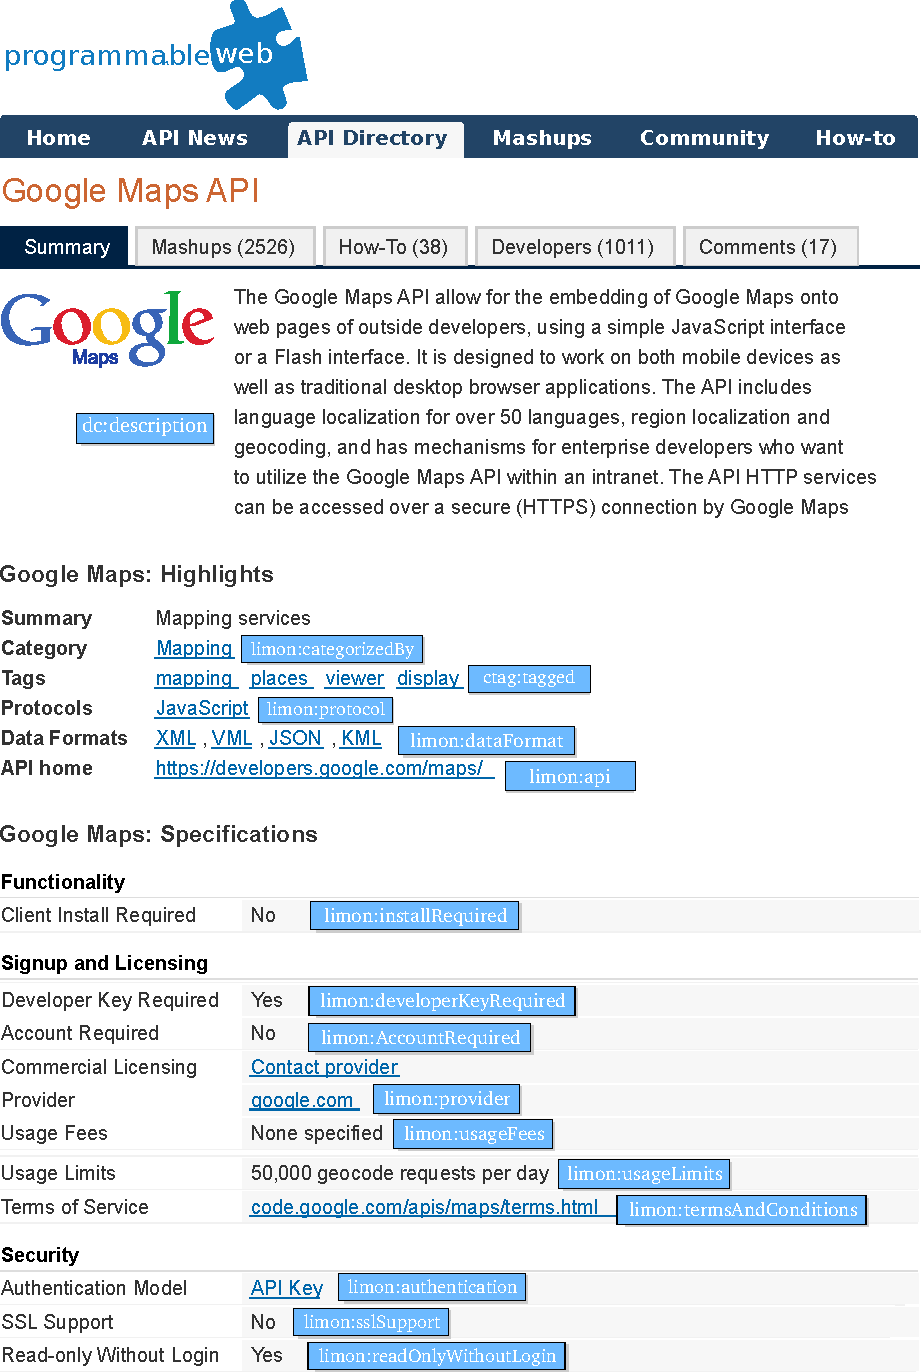
\includegraphics[height=600pt]{graphics/programmable_tags.pdf}
	\caption{Original site and corresponding LiMOn mapping}
	\label{fig:programmablewebgoogle}
\end{figure}

\lstinputlisting[style=listXML, caption=Full RDF of scrapped widget, label={lst:fullexamplerdf}]{code/www_programmableweb_com-api-google-maps.rdf}



\newpage
\section{Ranking algorithm}

The ranking algorithm needs to be executed by the administrator before accessing the OMR admin interface if we want to visualize the metrics corresponding to ranking. It could have done parallel to the scrapping process, but as explained in section \ref{sec:rankingmodule} in order to calculate in an accurate way the ranking indexes all the mash-ups need to be present at the same time because there is correlated information. In the same way, if a new service is discovered by Scrappy because we repeated the process  in section \ref{sec:autodiscovery} we will need to execute the ranking algorithm again.

Before executing the algorithm, it needs to have an instance of Scrappy running as a web server. This is explained in appendix \ref{sec:scrappyusermanual}.

The administrator user has to configure the configuration file configuration.properties (listing \ref{lst:rankingconfigfile}) and the run the algorithm .

\begin{lstlisting}[style=consola,label={lst:runranking}]
bash startRanking.sh
\end{lstlisting}


\begin{lstlisting}[style=consola, label={lst:rankingconfigfile},caption={Ranking algorithm configuration file}]
#OMR endpoint
omr=https://vsr-web.informatik.tu-chemnitz.de/omr-write/components/sparql

#Username
user=omr-client-upm

#Password
password=omr.client.upm.2012
\end{lstlisting}

\begin {table}[h]
\caption {Ranking algorithm execution statistics} \label{tab:rankingelapsedtime} 
\begin{center}
	\begin{tabular}{|c|c|}
		\hline \textbf{Elapsed time}                 	   & 7 hours and 4 minutes          \\ 
		\hline 
	\end{tabular} 
\end{center}
\end{table}

This process could take long time as showed in table \ref{tab:rankingelapsedtime}.

\begin{lstlisting}[style=listXML, label={lst:rdfranking}, caption={Ranking algorithm output}]
<limon:DegCent>0.82</omelette:rating>
<limon:ClosCent>4.21</omelette:rating>
<limon:RatSoc>131</omelette:rating>
\end{lstlisting}

\newpage
\section{OMR administrative interface}

After having the repository filled with all the services our purpose is to select those which we consider as interesting and also reject those which we don't want.
The administrator must enter the administrative interface (see appendix \ref{chap:omradmininstall} for installation and configuration).
In this scenario this is done by opening in the webbrowser the followind URL:
\begin{lstlisting}[style=consola]
http://lab.gsi.dit.upm.es/~pmoncada/omr-admin-pfc
\end{lstlisting}

The administrator will see the main view showed in figure \ref{fig:omradminmainview}.

\begin{figure}[h]
	\centering
	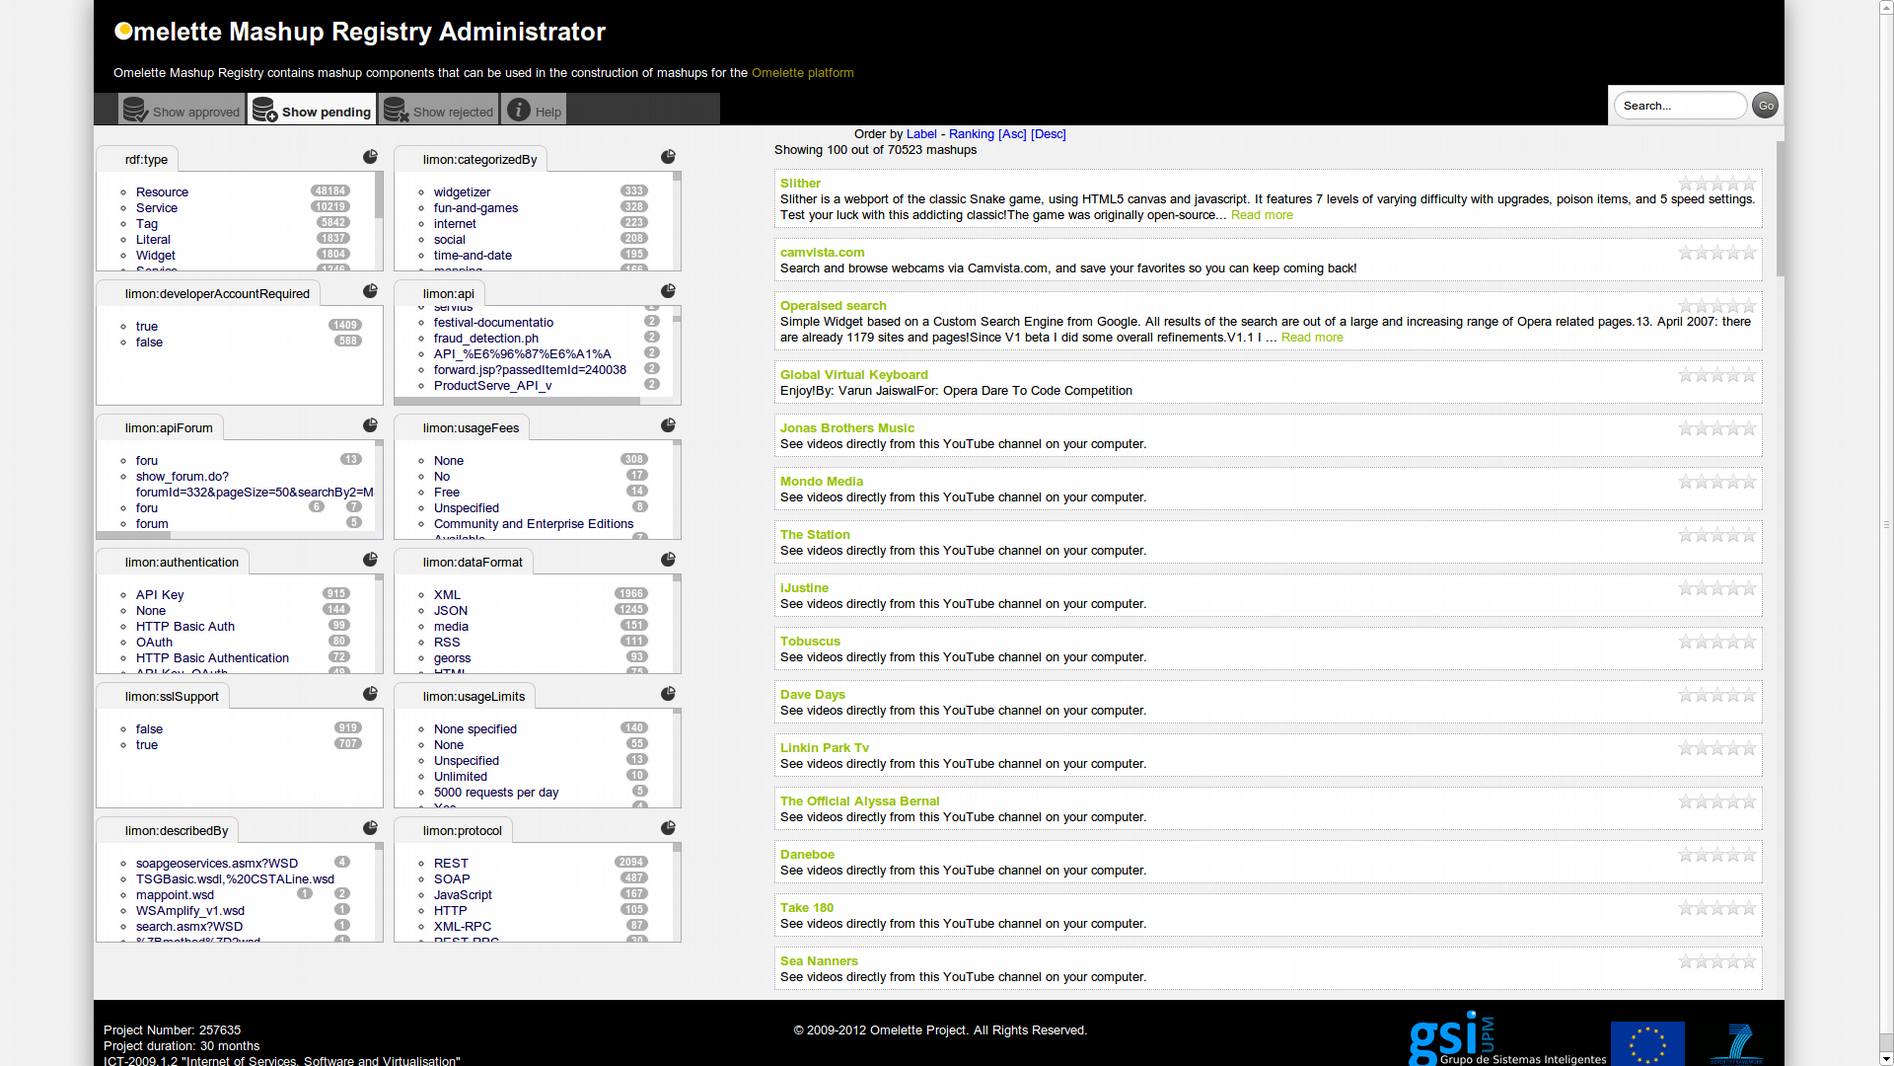
\includegraphics[width=400pt]{graphics/omr-admin-main.png}
	\caption{Main view OMR Administrator}
	\label{fig:omradminmainview}
\end{figure}


In the main view of the OMR Administrator, a menu is shown at the top:

\begin{figure}[h]
	\centering
	
\includegraphics[width=200pt]{graphics/admin-top-menu.png}
	\caption{OMR admin top menu}
	\label{fig:topmenuomr}
\end{figure}

\begin{description}
\item[Show approved] shows those mash-ups which have been selected by the
administrator as approved.
\item[Show pending] shows everything that that has been returned has the output of the
scrapping process.
\item[Show rejected] shows the lists of mash-ups that have been previously rejected by
the administrator.
\end{description}

\subsection{Available general actions}
\label{subsec:omravailableactions}
The following options will help the administrator to find those components he thinks of they are interesting or those who might be rejected.

\subsubsection{Filtering}
To filter using the filtering boxes click on a property from a filtering category.
Many filters can be selected at the same time. First select one of them, the view will refresh
with the new results. Then select next filter, the former filter will be sill selected, and results
will be filtered by many filters as chosen.

\textbf{Example}

We want add mash-ups compatible with \textit{JSON and XML } data formats and supporting \textit{REST, JavaScript and HTTP} protocols. To filter the mash-ups with this criteria, we select it in the facet boxes.

\begin{figure}[h]%
    \centering
    \subfloat[limon:protocol]{{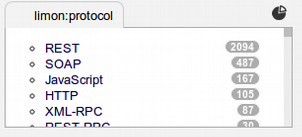
\includegraphics[width=4cm]{graphics/limon_protocol.png} }}%
    \qquad
    \subfloat[limon:dataFormat]{{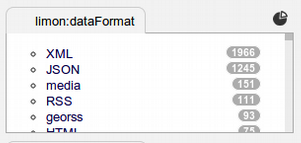
\includegraphics[width=4cm]{graphics/limon_dataformat.png} }}%
    \caption{Filtering by LiMOn properties}%
    \label{fig:limonfiltering}%
\end{figure}

\subsubsection{Searching}
The administrator user can use the search box to find a mash-up by name or description.

\textbf{Example}

We write "maps" in the search box (Figure \ref{fig:omradminsearchbox}), and the results are shown in the result area.

\begin{figure}[h]
	\centering
	
\includegraphics[width=100pt]{graphics/maps-search.png}
	\caption{OMR admin search box}
	\label{fig:omradminsearchbox}
\end{figure}

\subsubsection{Obtaining help}
If the administrator does not the meaning of anything appearing in the interface can consult the interactive help by mousing over the help icon.
\begin{figure}[h]
	\centering
	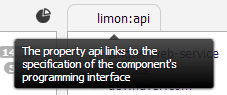
\includegraphics[width=150pt]{graphics/omr-admin-help.png}
	\caption{OMR admin help}
	\label{fig:omradminhelp}
\end{figure}

\subsubsection{Statistics}
\label{subsec:appendixstatistics}

The administrator might know how many mash-ups of a kind are added to the repository. When large amount of services are present is kind of difficult to handle this information. The administrator user can check this information in graphics presentation (Figure ref{fig:omradminseestatistics}).

\begin{figure}[h]
	\centering
	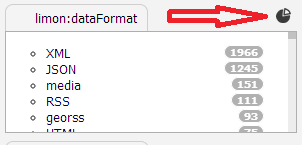
\includegraphics[width=150pt]{graphics/omr-admin-see-statistics.png}
	\caption{OMR see statistics}
	\label{fig:omradminseestatistics}
\end{figure}


\subsection{Reject a resource}

There are several reasons why we would like to reject various discovered mash-ups, such as the functionality of its is not related to our working lines or it was wrong scrapped in the automated discovery process (bad character encoding like in figure \ref{fig:badencoding}, mismatch of the information, etc). We could think just in deleting them from the system, but there is the possibility that we change our mind about this action in the future and we regret it. Also this avoids repeating the scrapping process from re-inserting the mashup again in the repository. This is way the admin interface will allow us to mark the mash-up as rejected as explained in section \ref{subsubsection:validationresourcearch}.

\begin{figure}[h]
	\centering
	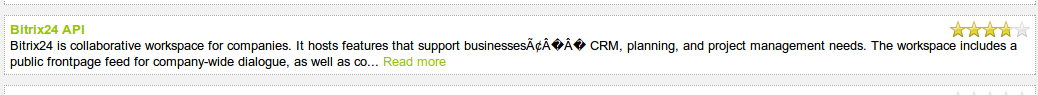
\includegraphics[width=400pt]{graphics/omr-bad-encoding.png}
	\caption{Bad charset encoding in widget description}
	\label{fig:badencoding}
\end{figure}

Before validating a resource we may want to know more information about it, and this can be done by visualizing the full content of the service. This must be done before validating, even if we are mostly sure about the component is the desired one, but sometimes as explained in the former paragraph there could be some problems in the scrapped information. The duty of the admin is to make sure the services that are validated are the correct ones.

The administrator can use the tools explained section \ref{subsec:omravailableactions} to get further information and help to complete the process. As an example the administrator could need extra information about the different fields and this can be achieved using the mouse-over functionality.

In our use case we want to have uniform types of mash-ups in the repository so the statistics diagrams provided by the admin interface would result very useful. We can find how to use them in section \ref{subsec:appendixstatistics}.

\subsection{Validating resource example}
As we saw in listing \ref{lst:fullexamplerdf} a service from Google Maps was scrapped, so let's try to find it in the admin interface. The easiest way would be to type "Google Maps API" in the search box and the result would be the desired one. But considering we don't know anything about the scrapped mashup this is not useful. Nevertheless we know some characteristics about a mash-up we need, which are:

\begin{itemize}
	\item It is a widget for maps.
	\item It must be compatible with XML and JSON data format.
	\item It must support javascript.
\end{itemize}

Doing a fast search just writing "maps" in the search box and after this selecting "JSON", "XML" and "Javascript" in the facet boxes the desired result (figure \ref{fig:googlemapsapi} will be showed on the right.

\begin{figure}[h]
	\centering
	
\includegraphics[width=400pt]{graphics/google-maps-api.png}
	\caption{Google maps api service in admin interface}
	\label{fig:googlemapsapi}
\end{figure}

To validate this service, the administrator has to click on the check box and then click on the \textit{validate} button to submit the data.

In order to understand the process of validating resources see section \ref{subsubsection:validationresourcearch}.

When we have selected and validated all the services we wanted, our task as administration user will be finished. This task can be resumed at any time if more needed services come out.

\section{Web developer interface}
This application is used by the developer user, who wants to find suitable services to build an application.
It is done using the OMR client interface through the web browser.

\begin{lstlisting}[style=consola,label={lst:runranking}]
http://krusti.gsi.dit.upm.es:8080/omr/
\end{lstlisting}

The interface of this application is much clearer as easier to use than the administrative one, as it is built for end users. Also the functionalities are not exactly the same, in this second search engine there are intelligent technologies as semantic search.

\begin{figure}[h]
	\centering
	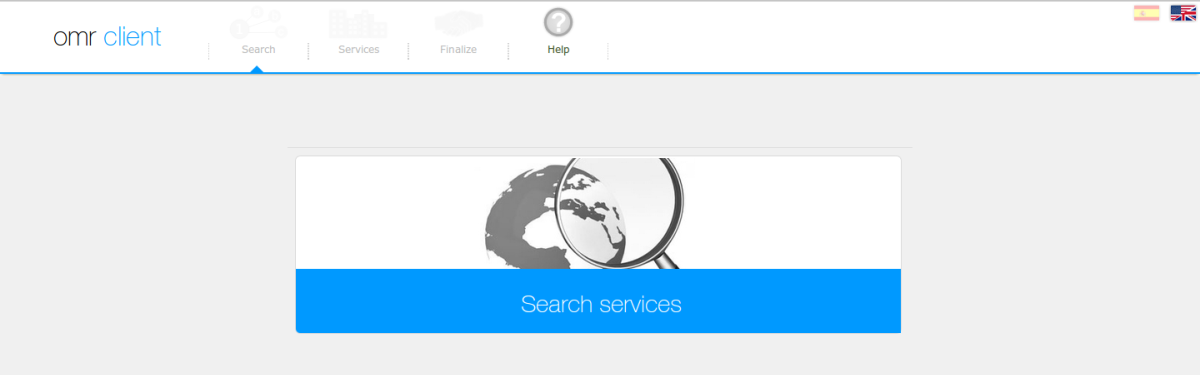
\includegraphics[width=400pt]{graphics/omr-client-main.png}
	\caption{OMR Developer interface main}
	\label{fig:searchservice}
\end{figure}


\textbf{Example}

Following the example exposed formerly, a developer wants to embed a map into an application to show the users interesting places. He doesn't know which one will better suit into his requirements. It must be a \textit{widget} and does not want to create a developer account.

The developer user accesses the interface and clicks on the "Search service" button (figure \ref{fig:searchservice}).

\begin{figure}[h]
	\centering
	
\includegraphics[width=300pt]{graphics/search-service.png}
	\caption{Search service button}
	\label{fig:searchservice}
\end{figure}

In the next step we can create a new search or select a search (figure \ref{fig:selectsearch}) we did before and we want to reuse it or refine it. The only difference will be that the form in next step will be filled or will be blank.

\begin{figure}[h]
	\centering
	
\includegraphics[width=300pt]{graphics/select-search.png}
	\caption{Select saved search or create a new one}
	\label{fig:selectsearch}
\end{figure}

Creating a new search will show us a fillable form which we will fill in according to our search criteria. 

\begin{figure}[h]
	\centering
	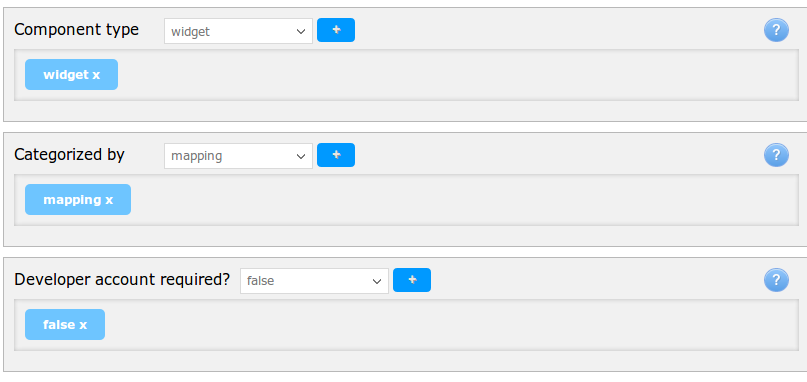
\includegraphics[width=400pt]{graphics/omr-client-filters.png}
	\caption{Select filters for the search}
	\label{fig:selectfilters}
\end{figure}

\begin{figure}[h]
	\centering
	
\includegraphics[width=300pt]{graphics/omr-client-show-results.png}
	\caption{Show results}
	\label{fig:selectsearch}
\end{figure}


\newpage

And after pressing the "Search results" the semantic search will be done in background by the semantic module and they will be presented as shown in figure \ref{fig:foundservices}. The first three services are marked with \textit{gold}, \textit{silver}, or \textit{bronze} medals which indicate that those are the best 3 services found by the semantic module. At the bottom the developer can see recommended services. These are services ordered by the ranking module having into account the social index.

\begin{figure}[h]
	\centering
	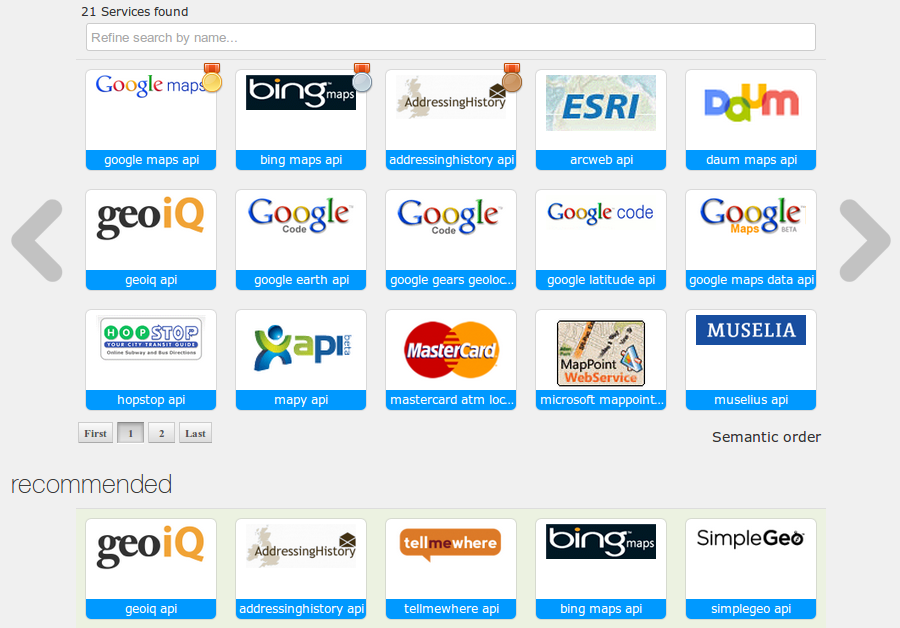
\includegraphics[width=300pt]{graphics/found-services.png}
	\caption{Found services by the semantic module}
	\label{fig:foundservices}
\end{figure}

We can extend the information (figure \ref{fig:extendedinfo}) and check if it satisfies us to finally select it as a candidate to use it in our application.

\begin{figure}[h]
	\centering
	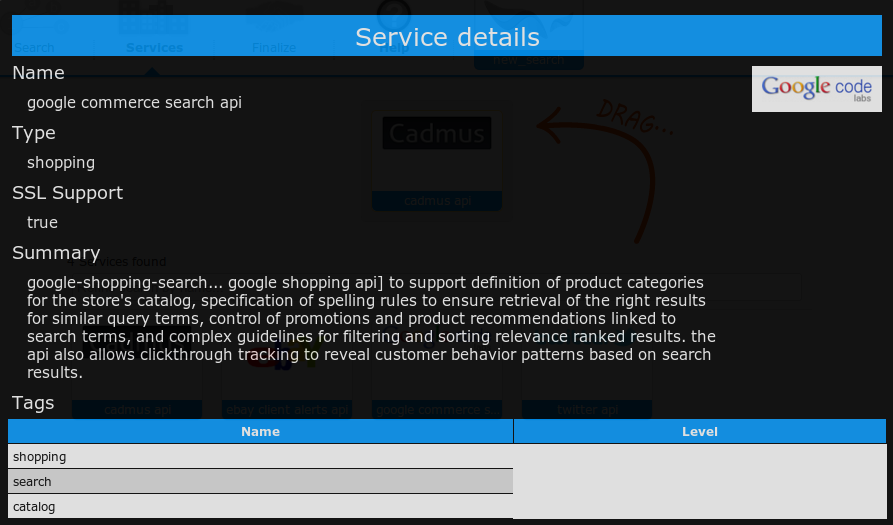
\includegraphics[width=300pt]{graphics/extended-info.png}
	\caption{Extended service info}
	\label{fig:extendedinfo}
\end{figure}

\section{Conclusions}

It is a very powerful search engine that enables real semantic search functionality to the final user, enabling search using natural language and offering similar results that suits into the user preferences that at a first instance he wouldn't have even thinked about.

The setting up of the scenario (filling in the repository and filtering) is quite slow but comparing it to the results given after is more than acceptable. The human intervention of an user administrator to filter the mash-ups gives the final user a great search experience which cannot be done by full automatic search engine of this characteristics.

